\documentclass[a4paper,11pt]{article}

\usepackage{../préambule}

\makeatletter
\renewcommand{\maketitle}{%
{\scriptsize colle dans ton cahier d'exercices} \vspace{0.5em}

	\begin{center}
		\LARGE
		\myuline{\@title}
		\vspace{1em}
	\end{center}
}
\makeatother

\title{Activité : Geogebra}
\date{}
\author{}

\begin{document}

\maketitle

\begin{exercice}\
	\begin{enumerate}
		\item Construit une figure en suivant les instructions ci-dessous :
		      \begin{enumerate}
			      \item Construit deux points A et B. Construit un segment passant par ces deux points.
			      \item Construit le cercle c de centre A passant par B.
		      \end{enumerate}
		\item Puis, utilise Geogebra pour afficher les longueurs suivantes :
		      \begin{enumerate}
			      \item La longueur [AB].
			      \item Le périmètre du cercle c.
		      \end{enumerate}
	\end{enumerate}
\end{exercice}

\begin{exercice}\

	Ouvre un tableur dans Geogebra, en sélectionnant \textit{Affichage → Tableur} dans le menu.

	Reproduit la tableau de la figure ci-dessous :

	\begin{center}
		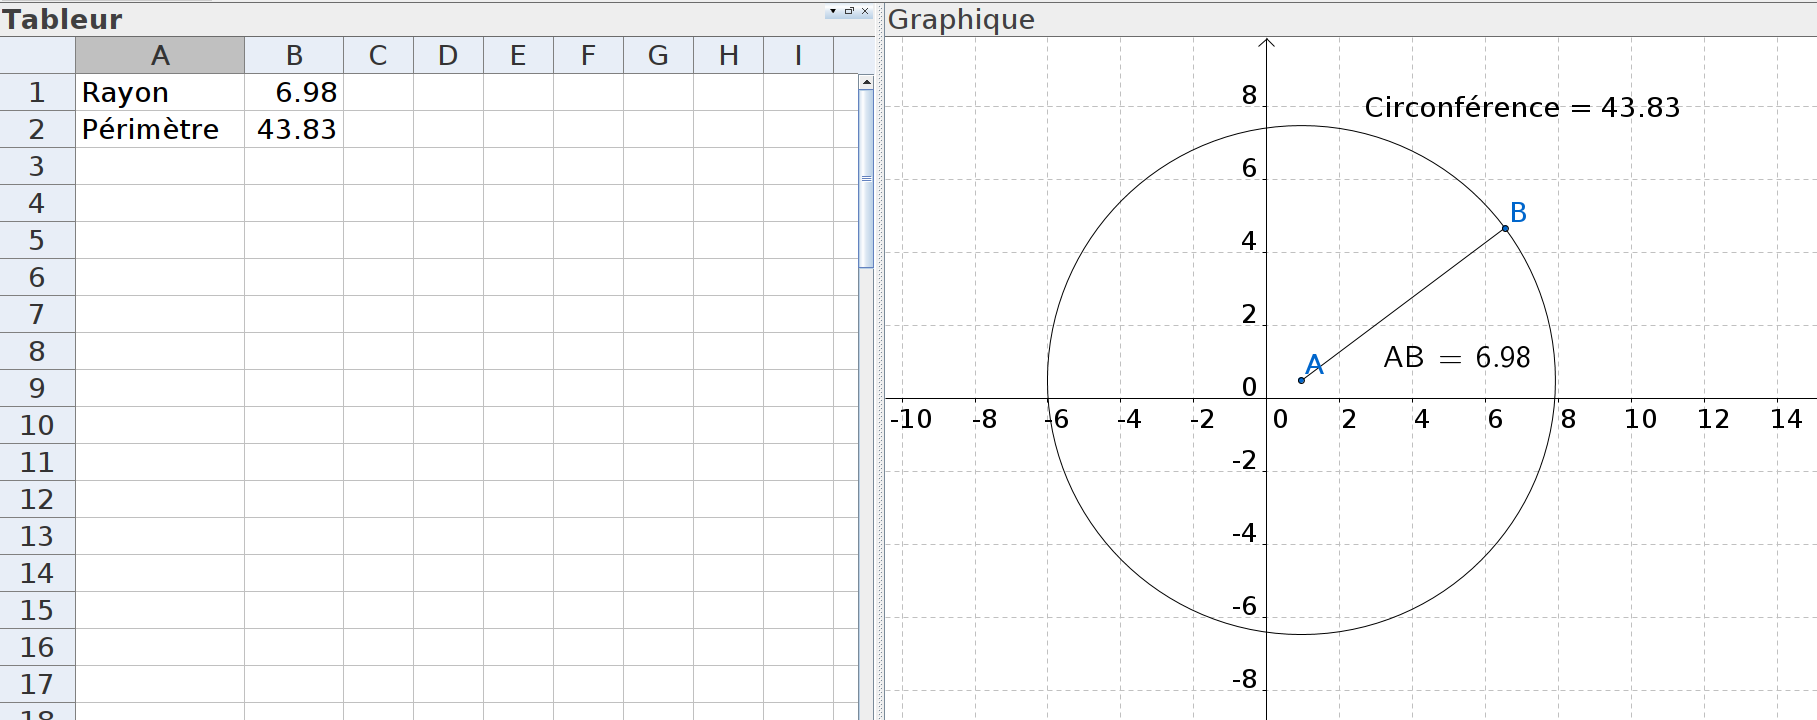
\includegraphics[width=0.85\linewidth]{Images/Activité - Geogebra - figure.png}
	\end{center}

	\begin{enumerate}
		\item Dans la deuxième colonne, note le rayon et le périmètre obtenus dans l'exercice 1.
		\item Bouge le point B, ou le point A. Note dans la troisième colonne les nouveaux rayon et périmètre.
		\item Change encore les positions pour une quatrième colonne.
		\item Enfin, dans la \textbf{troisième} ligne, pour chaque colonne, note le résultat du calcul
		      $$ \text{périmètre} ÷ \text{rayon} $$
		      \notebox {
			      Dans le tableur, la division se fait avec le signe /.
		      }
	\end{enumerate}
\end{exercice}

\begin{exercice}\

	On va maintenant utiliser les \textbf{formules} du tableur.

	\begin{enumerate}
		\item
	\end{enumerate}
\end{exercice}

\awesomebox[violet]{2pt}{\faRocket}{violet}{
	\textbf{Pour aller plus loin}
	\begin{itemize}
		\item Crée un segment, dont la longueur est le périmètre du cercle c.
		\item Peux-tu construire un cercle de périmètre 5 ?
	\end{itemize}
}

\end{document}